\section{Comparing plain GAN and Wasserstein GAN}

\subsection{Generator's and discriminator's architecture}

\begin{figure}[h]
	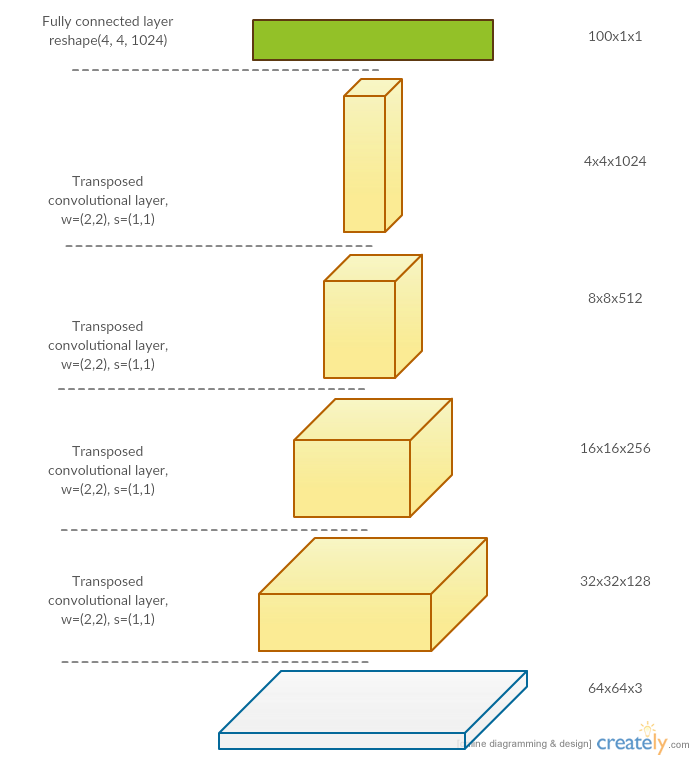
\includegraphics[width=0.5\textwidth]{figures/arc_gen}
	\caption{Architecture of the GAN used in this paper.}
	\label{fig:gan_arc}
\end{figure}
\subsection{Proposed evaluation method}
Unfortunately, the generative adversarial metric discussed in section~\ref{sec:gam} can not be applied to compare a plain GAN with a WGAN. This is due to the fact that output of a WGAN's discriminator can not be interpreted as a probability that sample is real. Therefore, we can not compute the $\epsilon(D_{WGAN}(x_{real}))$ and $\epsilon(D_{WGAN}(G_{GAN}(z)))$ terms of equation~\ref{eq:gam_real} and \ref{eq:gam_gen} respectively. I tried to use an approach inspired by GAM, but instead of plotting test results in terms of error rates on the test data set, I plotted discriminators' losses during the training process. Here is the summarized procedure: 
\begin{enumerate}
	\item Do several training steps of both the GAN and the WGAN.
	\item Log WGAN's discriminator performance 
		\begin{enumerate}
			\item Compute the WGAN discriminator's loss using images generated by the GAN's generator.
			\item Compute the WGAN discriminator's loss using its own generator
		\end{enumerate}	
	\item Log GAN's discriminator performance
		\begin{enumerate}
			\item Compute the GAN discriminator's loss using images generated by the WGAN's generator.
			\item Compute the GAN discriminator's loss using its own generator
		\end{enumerate}
	\item Go the step 1.
\end{enumerate}
Before taking a look at the results let us discuss possible outcomes of the procedure described above, which are visualized in figures~\ref{fig:cd_wgan_wins},~\ref{fig:cd_gan_wins},~\ref{fig:cd_dis_overfit},~\ref{fig:cd_gen_overfit}. At the end we would like to see a figure like~\ref{fig:cd_wgan_wins}. Here WGAN discriminator performs better when judging images produced by GAN's generator. On the other hand, GAN discriminator performs betters on the images of its own generator. In this case we can conclude that WGAN's generator was able to produce images that we harder to distinguish from the real ones by both discriminators and therefore it is likely that they have a better quality. The same is true in figure~\ref{cd:cd_gan_wins}, but here GAN's generator was able to produce better images. However, it also can not be the case that both generators overfit in respect to their own discriminators. This means, that they will be able to produce images that does not look better from a human perspective, but are tuned to fool the respective discriminator. In this case we will see graphs like in figure~\ref{fig:cd_gen_overfit}. It is also possible that discriminators overfit in a sense that instead of analyzing the structure of real images they remember peculiarities present in the images produced by their generators. In this scenario plots will resemble those shown in figure~\ref{fig:cd_dis_overfit}.

	\begin{figure}[h] 
		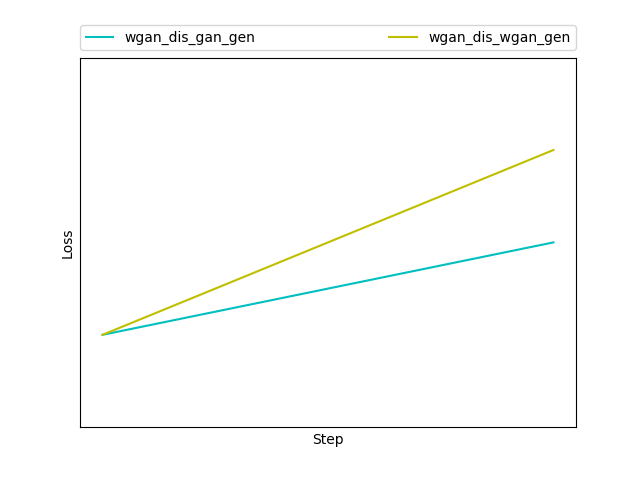
\includegraphics[width=0.5\textwidth]{figures/wgan_wins_wgan_dis_gan_gen}
		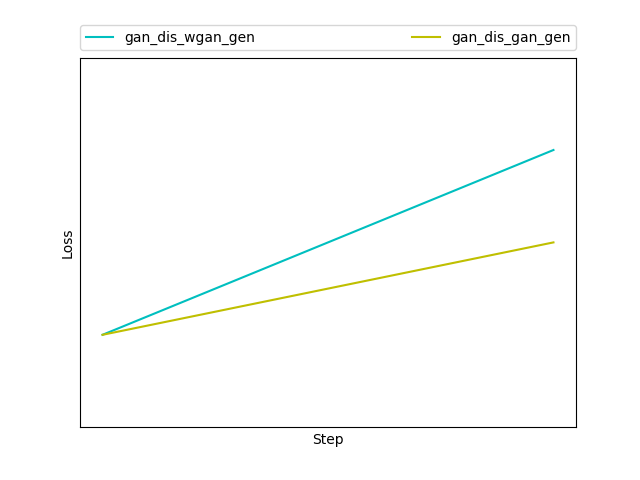
\includegraphics[width=0.5\textwidth]{figures/wgan_wins_gan_dis_wgan_gen}
		\caption{Both WGAN and GAN discriminators losses are bigger when competing against WGAN generator.}
		\label{fig:cd_wgan_wins}
	\end{figure}
	\begin{figure}[h] 
		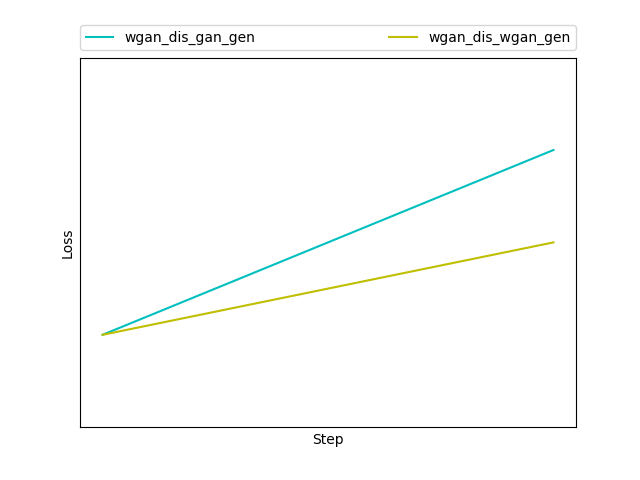
\includegraphics[width=0.5\textwidth]{figures/gan_wins_wgan_dis_gan_gen}
		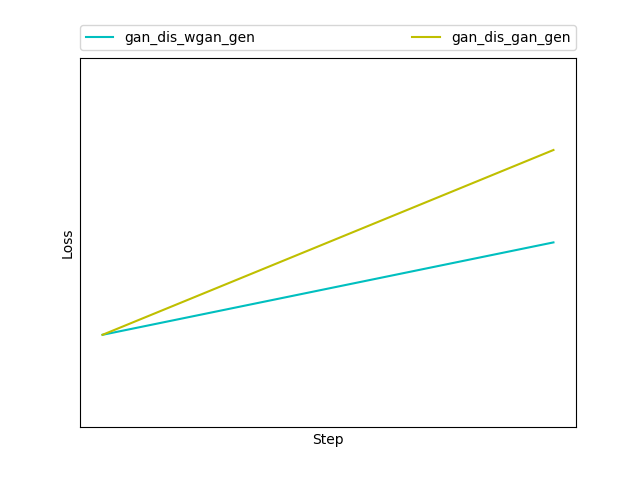
\includegraphics[width=0.5\textwidth]{figures/gan_wins_gan_dis_wgan_gen}
		\caption{Both WGAN and GAN discriminators losses are bigger when competing against GAN generator.}
		\label{fig:cd_gan_wins}
	\end{figure}
	\begin{figure}[h] 
		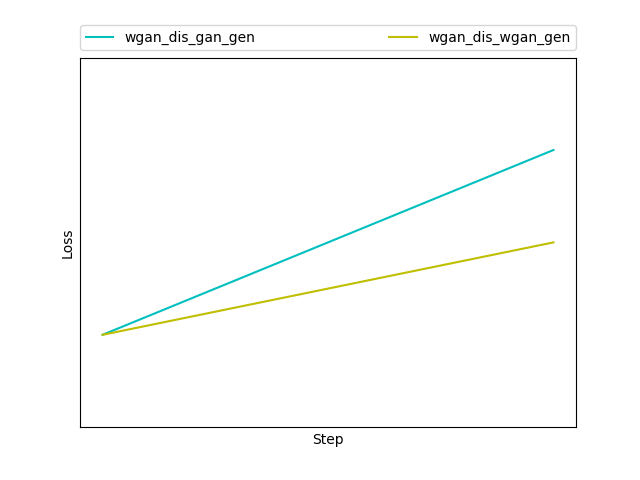
\includegraphics[width=0.5\textwidth]{figures/dis_overfit_wgan_dis_gan_gen}
		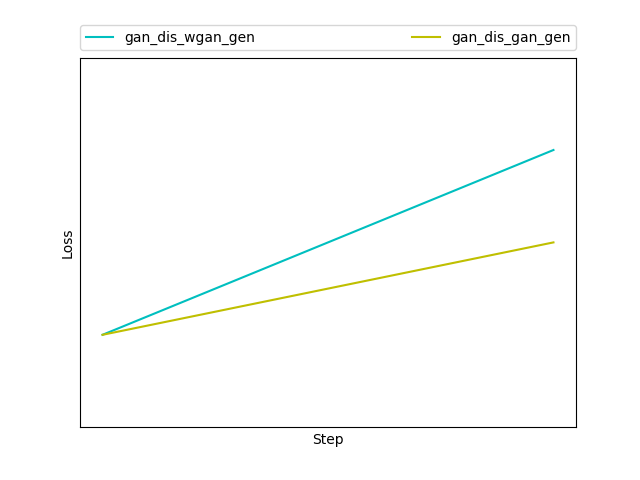
\includegraphics[width=0.5\textwidth]{figures/dis_overfit_gan_dis_wgan_gen}
		\caption{Both WGAN and GAN discriminators losses are bigger when competing against each other's generator. A sign that discriminators overfit against own generators.}
		\label{fig:cd_dis_overfit}	
	\end{figure}
	\begin{figure}[h] 
		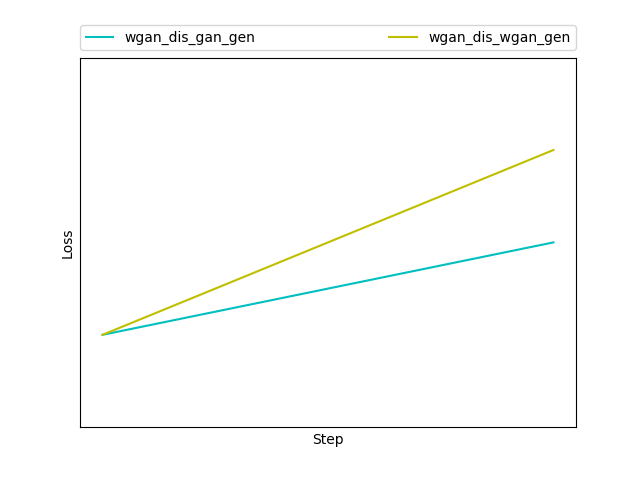
\includegraphics[width=0.5\textwidth]{figures/gen_overfit_wgan_dis_gan_gen}
		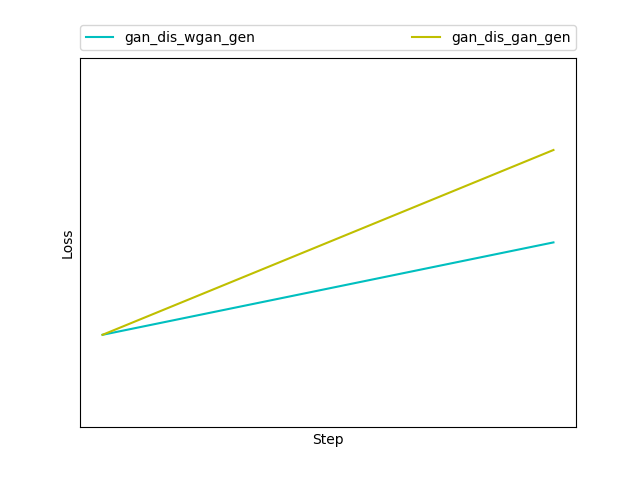
\includegraphics[width=0.5\textwidth]{figures/gen_overfit_gan_dis_wgan_gen}
		\caption{Both WGAN and GAN discriminators losses are bigger when competing against own generator. A sign that generators overfit against own discriminators.}
		\label{fig:cd_gen_overfit}
	\end{figure}

Note that particular result can happen due to the initialization of weight in a network. Therefore to draw any conclusion experiments have to be conducted multiple times. 

\subsection{Results}
 Results of applying the modified generative adversarial metric are shown in figure~\ref{fig:cd_wgan_vs_gan}. As we can see, after a few training step GAN's generator was able to label all images produced by the WGAN's generator as fake. On the other hand WGAN's discriminator also performed worse against its own generator. This suggests that generators may have overfit with the respect to their own discriminators. 
\begin{figure}[h]
	\begin{subfigure}[b]{0.5\textwidth}
		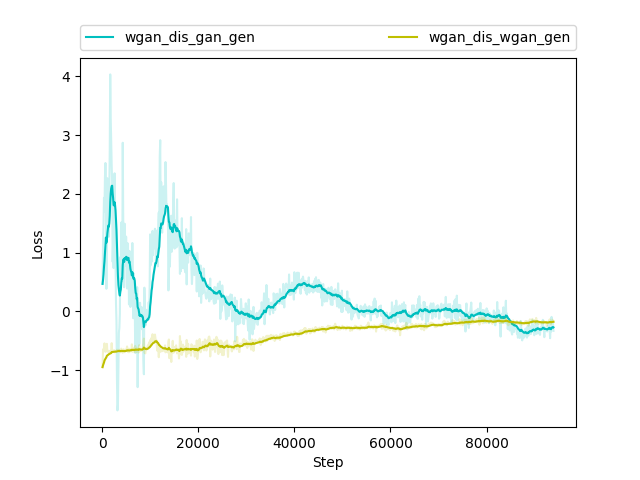
\includegraphics[width=\textwidth]{figures/wgan_dis_gan_gen}
	\end{subfigure}
	\begin{subfigure}[b]{0.5\textwidth}
		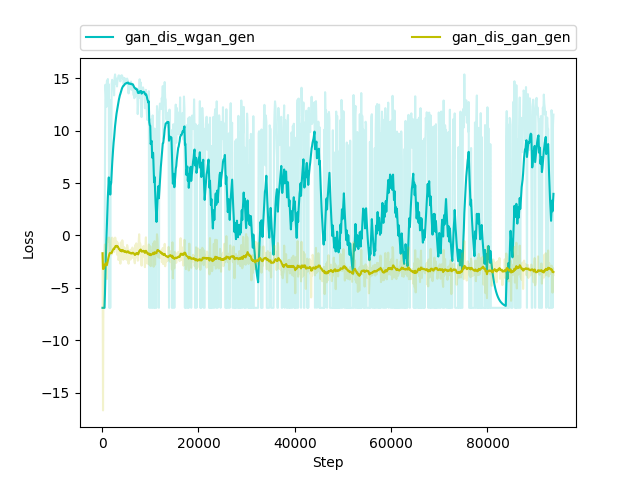
\includegraphics[width=\textwidth]{figures/gan_dis_wgan_gen}
	\end{subfigure}
	\caption{Results of applying the modified adversarial metric on a GAN and a WGAN. As we can see GAN's discriminator almost constantly performs worse when judging images produced by WGAN's generator, on the other hand WGAN's discriminator performs equally well on both generators.}
	\label{fig:cd_wgan_vs_gan}
\end{figure}

\begin{figure}[h]
	\begin{subfigure}[b]{0.5\textwidth}
		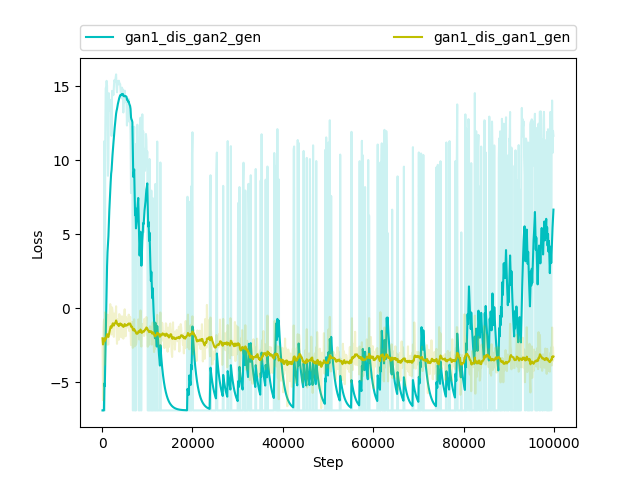
\includegraphics[width=\textwidth]{figures/gan1_dis_gan2_gen}
	\end{subfigure}
	\begin{subfigure}[b]{0.5\textwidth}
		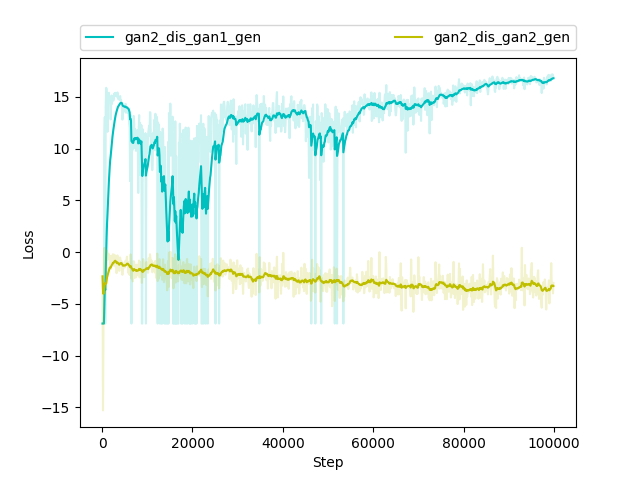
\includegraphics[width=\textwidth]{figures/gan2_dis_gan1_gen}
	\end{subfigure}
	\caption{Results of applying the modified adversarial metric on two GANs. Both discriminators can better distinguish images from their own generators}.
	\label{fig:cd_gan_vs_gan}
\end{figure}

To further investigate this hypothesis I have used the same metric to compare two GAN's. The corresponding results are shown in figure~\ref{fig:cd_gan_vs_gan}. Also in this setup both discriminators can distinguish images generated by a foreign generator 100\% of the time. The same is true for WGANs as shown in figure~\ref{fig:cd_wgan_vs_wgan}.
\begin{figure}[h]
	\begin{subfigure}[b]{0.5\textwidth}
		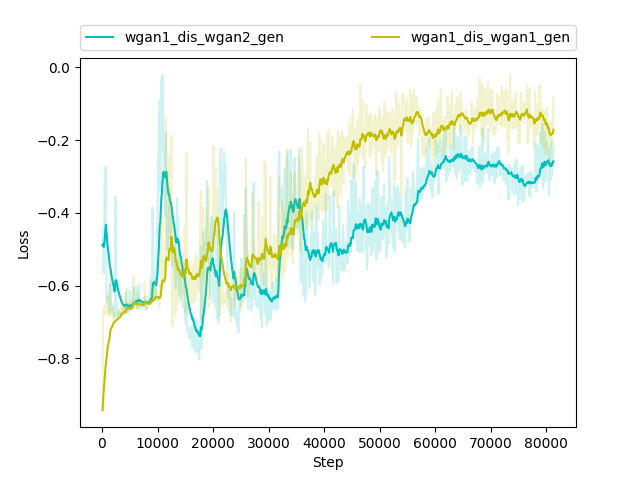
\includegraphics[width=\textwidth]{figures/wgan1_dis_wgan2_gen}
	\end{subfigure}
	\begin{subfigure}[b]{0.5\textwidth}
		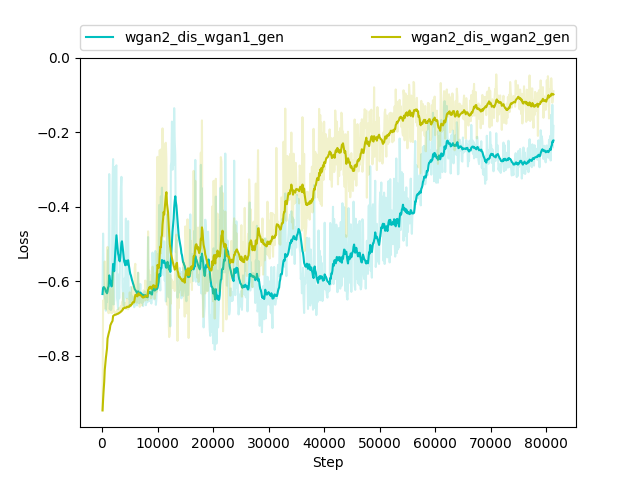
\includegraphics[width=\textwidth]{figures/wgan2_dis_wgan1_gen}
	\end{subfigure}
	\caption{Results of applying the modified adversarial metric on two WGANs. Both discriminators can better distinguish images from the foreign generator}.
	\label{fig:cd_wgan_vs_wgan}
\end{figure}

So we can conclude that by both GAN and WGAN generators are able to exploit the flows in discriminators to generate images that do not have better quality but are able to deceive the discriminator. To explore the decision boundary learned by a GAN discriminator we can conduct the following experiment. Once a discriminator is fully trained we can search for an image which discriminator will confidently identify as real. We can do it by using gradient descent over image space using the output of the discriminator as a loss function. However, using output directly can will result in a very slow learning, because the output of discriminator on a newly initialized random image will be almost zero. Therefore, sigmoid used as an activation in the last layer will be saturated and gradient will vanish. Instead, I used output before activation. Of coarse, the discriminators output is not a convex function and has numerous local maxima. But by conducting search multiple times with different initial images we have a chance to find a maxima that will give us a confidence near one. In practice it turned out that discriminator's decision boundary has lots of isolated regions where its confidence is equal to one. However, these regions are so small that after saving found image, the error introduced when converting each pixel value from floats to bytes already forces image to lie outside of the region. This is demonstrated in figure~\ref{fig:found_image_with_noise}. This experiment suggest that a discriminator learns not only a manifold containing faces in the space of possible images, but has many local peaks scattered over the whole image space. This can happen due to the fact that discriminator never has a chance to observe the whole image space, but rather sees only small portion of it depicted in the real images and images produced by a generator. Therefore the discriminator has no chance to learn what is the probability of other points.  

\begin{figure}[h]
	\begin{subfigure}[b]{0.5\textwidth}
		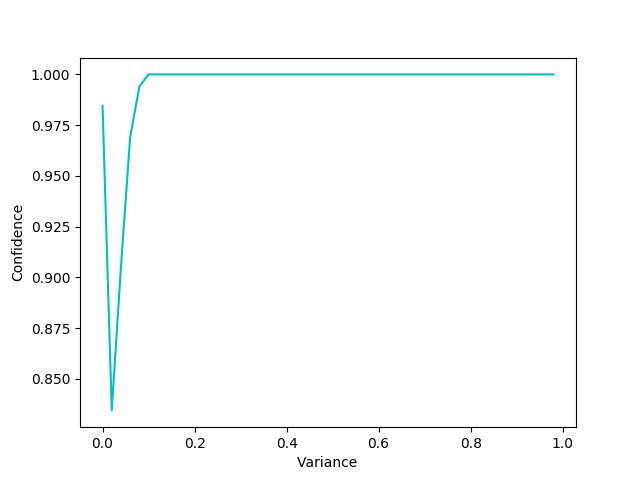
\includegraphics[width=\textwidth]{figures/diversity_gan2_real_dis_real_imgs_plot}
	\end{subfigure}
	\begin{subfigure}[b]{0.5\textwidth}
		\centering
		
\includegraphics[width=0.45\textwidth]{figures/diversity_gan2_real_dis_real_imgs_var0}
		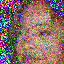
\includegraphics[width=0.45\textwidth]{figures/diversity_gan2_real_dis_real_imgs_var30}
		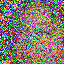
\includegraphics[width=0.45\textwidth]{figures/diversity_gan2_real_dis_real_imgs_var50}
		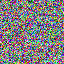
\includegraphics[width=0.45\textwidth]{figures/diversity_gan2_real_dis_real_imgs_var100}
	\end{subfigure}
	\caption{Visualization of how GAN discriminator's confidence changes when we add Gaussian noise to a real image sample.}
	\label{fig:changed_real_image_real_dis}
\end{figure}

\begin{figure}[h]
	\begin{subfigure}[b]{0.5\textwidth}
		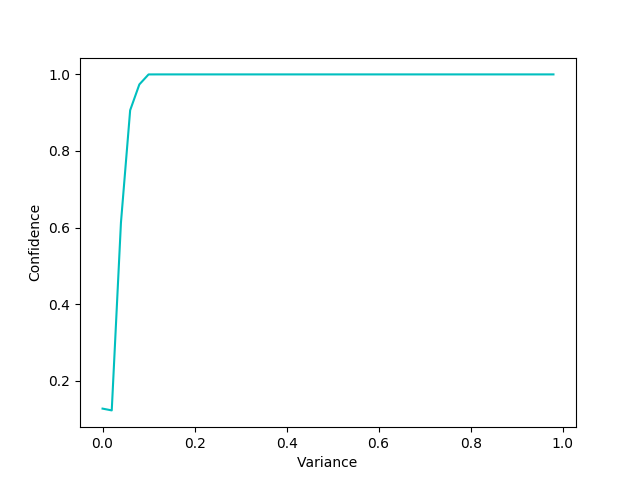
\includegraphics[width=\textwidth]{figures/diversity_gan2_fake_dis_gen_images_plot}
	\end{subfigure}
	\begin{subfigure}[b]{0.5\textwidth}
		\centering
		
\includegraphics[width=0.45\textwidth]{figures/diversity_gan2_fake_dis_gen_images_var_0}
		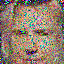
\includegraphics[width=0.45\textwidth]{figures/diversity_gan2_fake_dis_gen_images_var_30}
		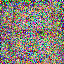
\includegraphics[width=0.45\textwidth]{figures/diversity_gan2_fake_dis_gen_images_var_50}
		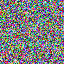
\includegraphics[width=0.45\textwidth]{figures/diversity_gan2_fake_dis_gen_images_var_90}
	\end{subfigure}
	\caption{Visualization of how GAN discriminator's confidence changes when we add Gaussian noise to a real image sample.}
	\label{fig:changed_gen_image_fake_dis}
\end{figure}

\begin{figure}[h]
	\begin{subfigure}[b]{0.5\textwidth}
		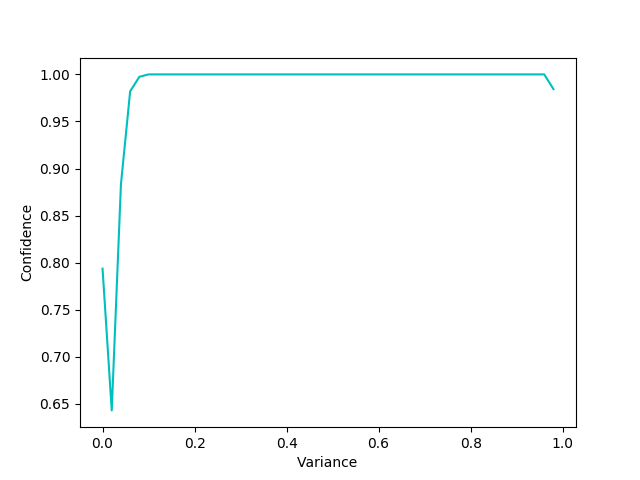
\includegraphics[width=\textwidth]{figures/diversity_gan2_real_dis_gen_images_plot}
	\end{subfigure}
	\begin{subfigure}[b]{0.5\textwidth}
		\centering
		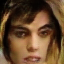
\includegraphics[width=0.45\textwidth]{figures/diversity_gan2_real_dis_gen_imgs_var0}
		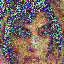
\includegraphics[width=0.45\textwidth]{figures/diversity_gan2_real_dis_gen_imgs_var30}
		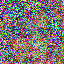
\includegraphics[width=0.45\textwidth]{figures/diversity_gan2_real_dis_gen_imgs_var50}
		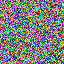
\includegraphics[width=0.45\textwidth]{figures/diversity_gan2_real_dis_gen_imgs_var90}
	\end{subfigure}
	\caption{Visualization of how GAN discriminator's confidence changes when we add Gaussian noise to a real image sample.}
	\label{fig:changed_gen_image_real_dis}
\end{figure}

\begin{figure}
	\begin{subfigure}[b]{0.5\textwidth}
		\centering
		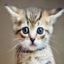
\includegraphics[scale=1]{figures/random_images_fake_1}
		
\includegraphics[scale=1]{figures/random_images_fake_2}
		\caption{The images that the GAN discriminator considered fake.}
	\end{subfigure}
	\begin{subfigure}[b]{0.5\textwidth}
		\centering
		
\includegraphics[scale=1]{figures/random_images_real_1}
		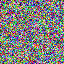
\includegraphics[scale=1]{figures/random_images_real_2}
		\caption{The images that the GAN discriminator considered real.}
	\end{subfigure}
\end{figure}


